\begin{solution}
\begin{enumerate}[label = (\alph*)]
    \item I simulate the model for \(T = 5000\) and \(N = 20\) and estimate the Fama-Macbeth estimator for a window of \(t = 100, 200,  \dots, T\). Figure~\ref{fig:beta_fm_a} shows the results for the traditional and the demeaned estimator. As we can see, the demeaned estimator does converges towards the true value of \(\beta\) as \(T\) increases. However, the traditional estimator does not converge, as explained in item (d).
    \begin{figure}[!htbp]
        \centering
        \includegraphics[width=0.6\textwidth]{../../images/beta_fm_a}
        \caption{Fama-MacBeth Estimator}
        \label{fig:beta_fm_a}
    \end{figure}

    \item  After removing the firm fixed effect from \(x_{it}\), the traditional estimator seems to be converging towards the true value as \(T\) increases as seen in Figure~\ref{fig:beta_fm_b}. The demeaned estimator behaves identically to the previous case.
    \begin{figure}[!htbp]
        \centering
        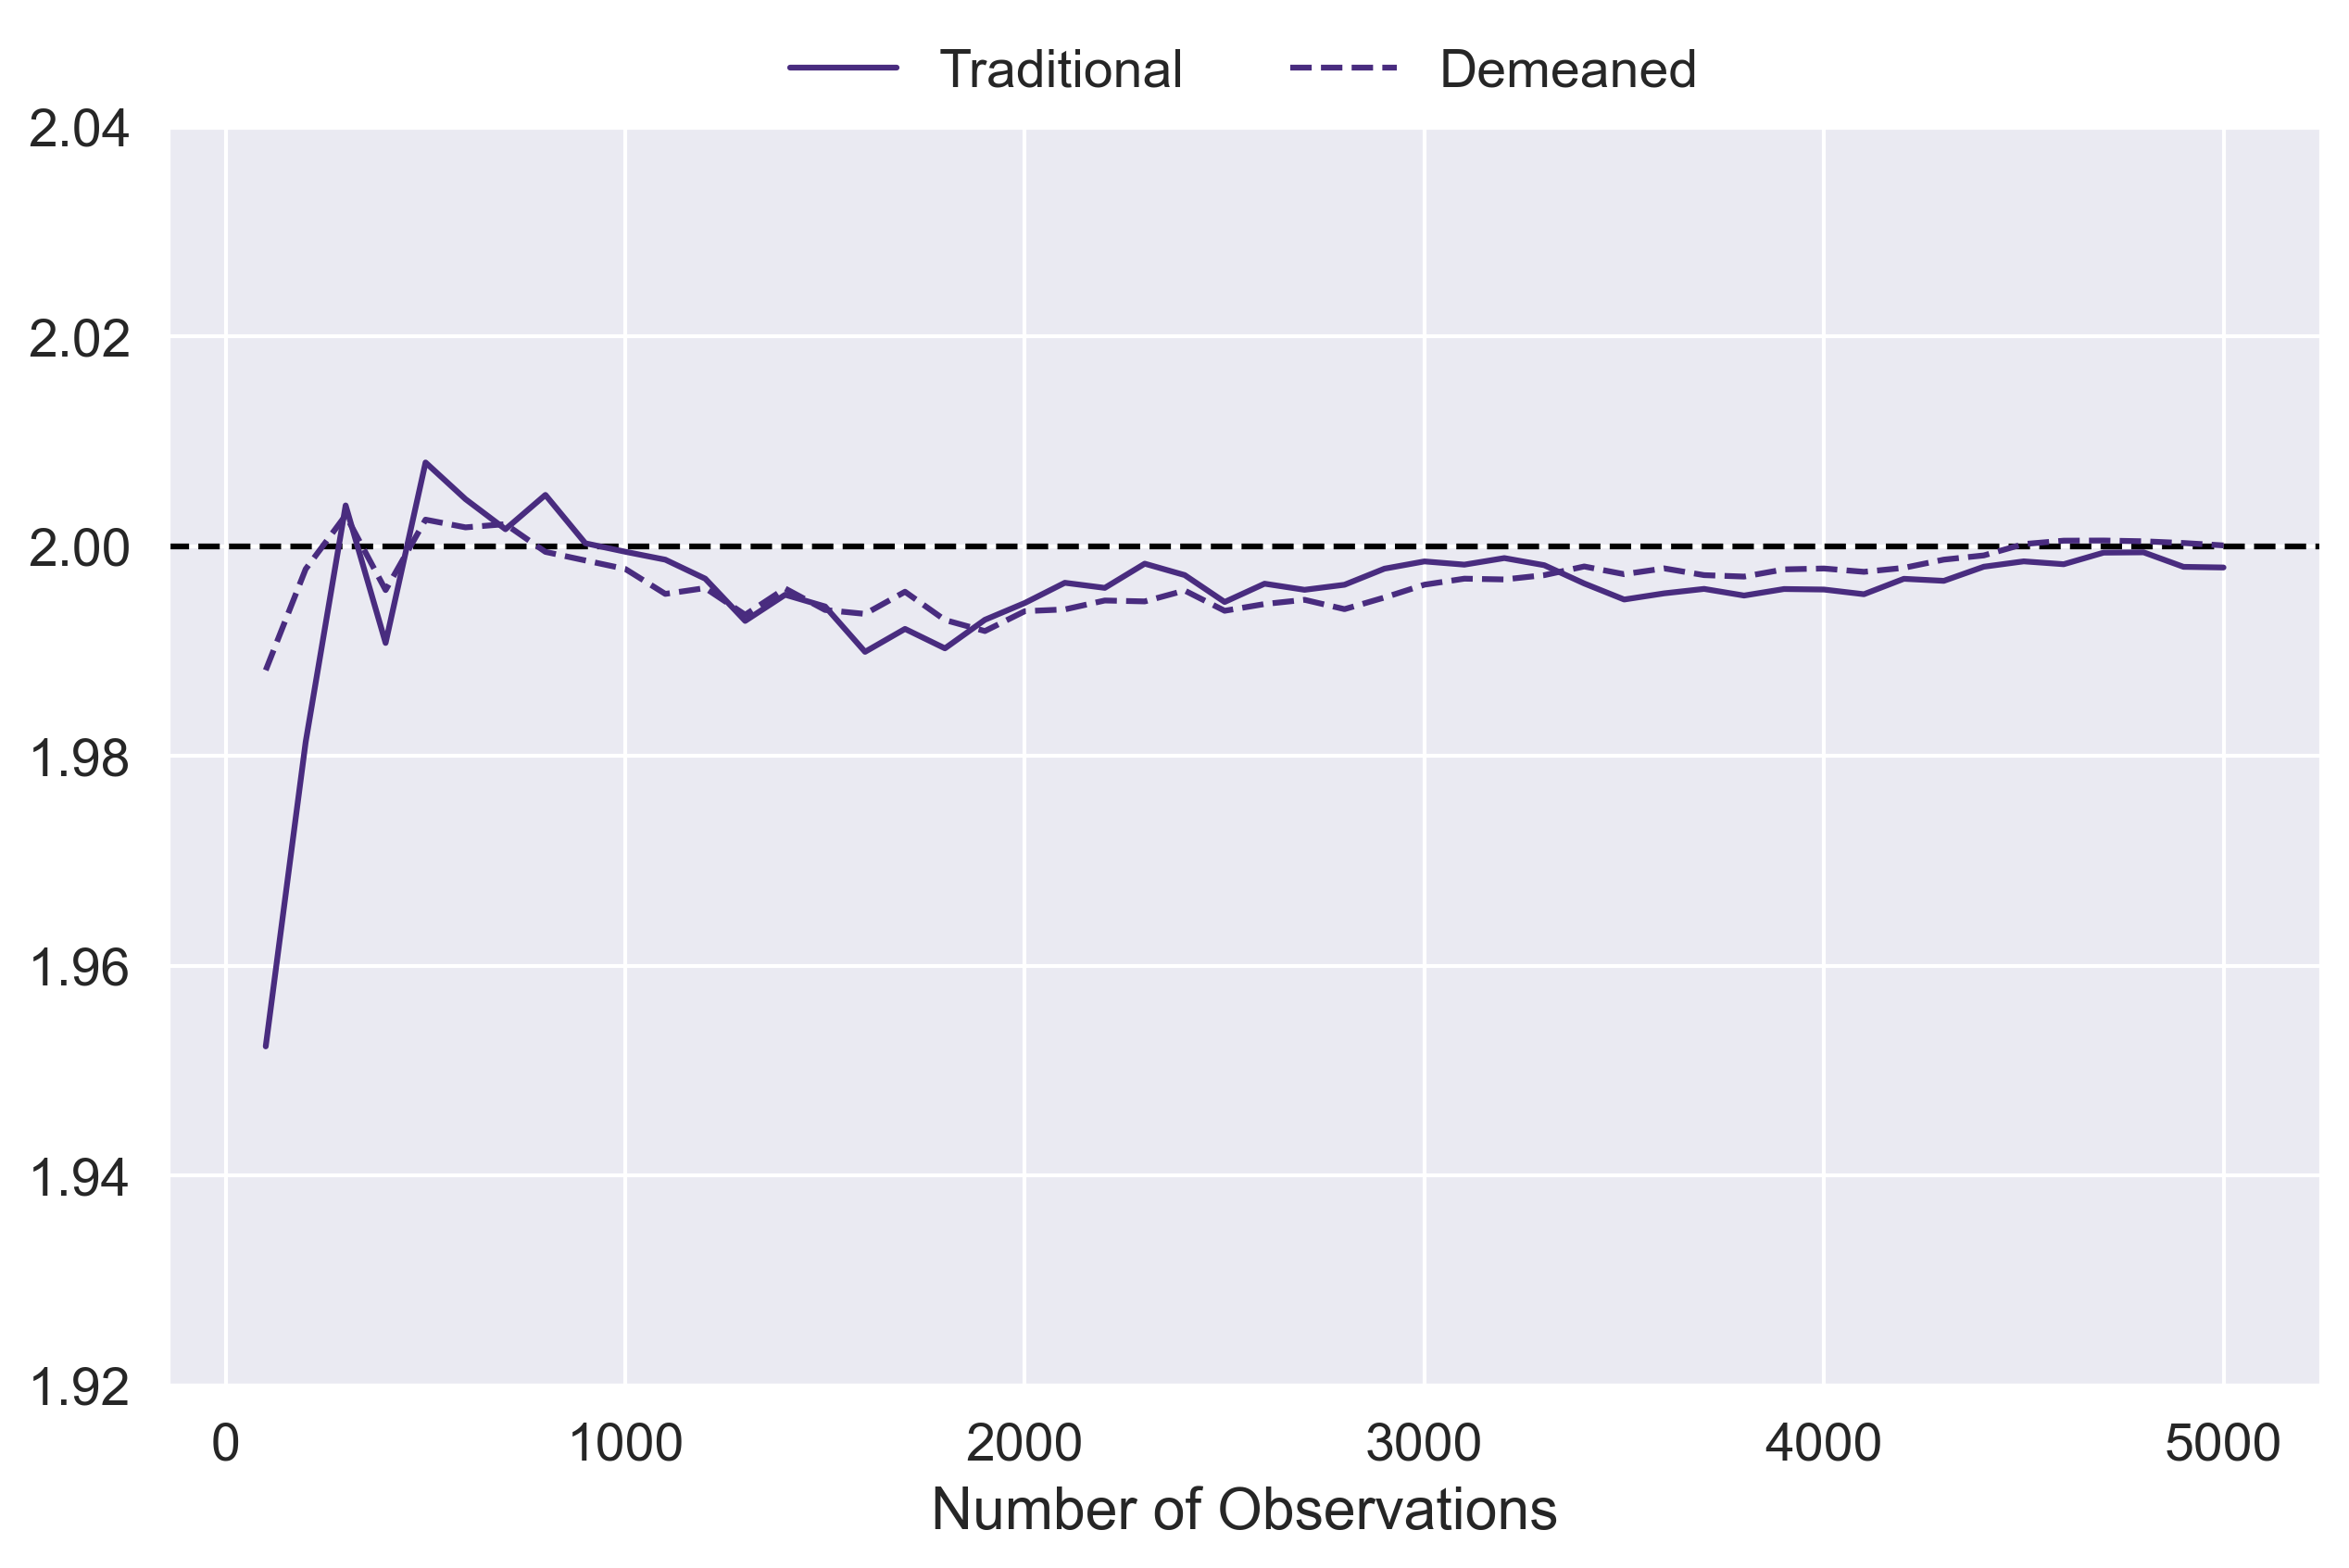
\includegraphics[width=0.6\textwidth]{../../images/beta_fm_b}
        \caption{Fama-MacBeth Estimator (\(\mu_i = 0\))}
        \label{fig:beta_fm_b}
    \end{figure}        

    \item After removing the fixed effect of the error term, the traditional estimator still looks consistent. See Figure~\ref{fig:beta_fm_c}. The demeaned is consistent as always. Again, the demeaned estimator is identical to the previous cases.
    \begin{figure}[!htbp]
        \centering
        \includegraphics[width=0.6\textwidth]{../../images/beta_fm_c}
        \caption{Fama-MacBeth Estimator (\(\gamma_i = 0\))}
        \label{fig:beta_fm_c}
    \end{figure}

    \item  We need to consider the following assumption:
    \begin{assump}
        \label{assump:min_eigen}
        The minimum eigenvalue of \(\sum_i x_{it}x_{it}^\prime\) is bounded from below.
    \end{assump}
    This implies that the inverse of \(\sum_ix_{it}x_{it}^\prime\) always exist so that \(\wh\beta_t\) is always defined. Moreover, it allow us to form an upper bound for the inverse across \(t\). \\
    We start by showing the consistency of the \textit{Traditional FM} estimator. Consider the \emph{fixed-t} estimator \(\wh\beta_t\):
    \begin{align*}
        \wh\beta_t & = \bp{\sum_i x_{it}x_{it}^\prime}^{-1}\bp{\sum_i x_{it}y_{it}} \\
        & = \beta + \bp{\sum_i x_{it}x_{it}^\prime}^{-1}\bp{\sum_i x_{it}\varepsilon_{it}}
    \end{align*}
    Therefore the FM estimator takes the average over \(t\) of \(\wh\beta_t\)
    \begin{align*}
        \wh\beta^{(T)}_{FM} = \beta + \frac{1}{T}\sum_t\bp{\sum_i x_{it}x_{it}^\prime}^{-1}\bp{\sum_i x_{it}\varepsilon_{it}}
    \end{align*}
    From Assumption \ref{assump:min_eigen}, we can bound this from above by
    \[
        \wh\beta^{(T)}_{FM}-\beta \leq M\frac{1}{T}\sum_t\sum_i x_{it}\varepsilon_{it}
    \]
    where \(M\) is the upper bound for the inverse of \(\sum_i x_{it}x_{it}^\prime\). \\
    Using equation \ref{eq:x_dgp}:
    \begin{align*}
        \label{eq:fm_consistency}
        \wh\beta^{(T)}_{FM} - \beta & \leq M\frac{1}{T}\sum_t\sum_i \bp{\mu_i+\eta_{it}}\bp{\gamma_i+\nu_{it}} \\
        & \leq M\frac{1}{T}\sum_t\sum_i\bp{\mu_i\gamma_i + \mu_i\nu_{it} + \gamma_i\eta_{it} + \eta_{it}\nu_{it}} \\
        & \leq M\sum_i\mu_i\gamma_i + o_p(1)
    \end{align*}
    Where the last line follows from the independence of \((\mu_i, \gamma_i, \eta_{it}, \nu_{it})\). Therefore the consistency of the FM estimator depends on the interaction of the fixed effects of \(x\) and \(\varepsilon\). 
    
    In case (b) and (c), we have that either \(\mu_i = 0\) or \(\gamma_i = 0\), so the first term in \eqref{eq:fm_consistency} disappears and the Traditional FM estimator is consistent. In (a), both terms are non-zero, so we don't necessarily have consistency. \\

    The consistency of the \textit{Demeaned FM} estimator follows the same procedure. When we demean our variables in across \(T\), we remove the firm fixed effects in both \(x_{it}\) and \(\varepsilon_{it}\). Therefore the term \(\sum_i \mu_i\gamma_i\) disappears and the estimator is consistent in all cases. To see that simply note that:
    \begin{align*}
        \wt x_{it} & \coloneqq x_{it} - \frac{1}{T}\sum_t x_{it} \\
        & = \mu_i + \eta_{it} - \frac{1}{T}\sum_t \bp{\mu_i + \eta_{it}} \\
        & = \mu_i - \mu_i + \eta_{it} - \frac{1}{T}\sum_t\eta_{it} \\
        & = \wt\eta_{it}
    \end{align*}
    Equivalently, \(\wt y_{it} = \beta\wt x_{it} + \wt\varepsilon_{it}\) with \(\wt\varepsilon_{it} = \wt \nu_{it}\). This equation has no firm fixed effect so \(\wh\beta^{(T)}_{DFM}\) is always consistent. 
    
    \item Similarly to (d), if there are time fixed effects, then the demeaning of \(\wh\beta^{(T)}_{DFM}\) does not remove the fixed effect. \\
    For the traditional estimator we then have, similarly to the derivations above,
    \begin{align*}
        \wh\beta^{(T)}_{FM} - \beta & \leq M \frac{1}{T}\sum_t\sum_i \bp{\delta_t+\eta_{it}}\bp{\psi_t+\nu_{it}} \\
        & \leq M\frac{1}{T}\sum_t\bp{\delta_t\psi_t + \delta_t\sum_i\nu_{it} + \psi_t\sum_i\eta_{it} + \sum_i\eta_{it}\nu_{it}} \\
        & \leq M\frac{1}{T}\sum_t \delta_t\psi_t + o_p(1)
    \end{align*}
    Therefore both estimator are consistent if the time fixed effects of \(x_{it}\) and \(\varepsilon_{it}\) are uncorrelated.

    \item I show that the estimated variance of the FM is unbiased under the following assumptions:
    \begin{assump}
        \label{assump:no_fe}
        There is no firm fixed effects in \(x_{it}\) or \(\varepsilon_{it}\)
    \end{assump}
    which is the case of (b) and (c) or if the variables are demeaned. \\
    Let \(p_{it} \coloneqq \bp{\sum_i x_{it}x_{it}^\prime}^{-1}x_{it}\). Then we can rewrite 
    \[
        \wh\beta_t = \beta + \sum_i p_{it}\varepsilon_{it}
    \]
    The considered DGP is the one in \eqref{eq:x_dgp} with firm fixed effects only and \(\varepsilon_{it}\) and \(x_{is}\) are independent for every \((t,s)\). We first consider the variance of the traditional FM estimator. 
    \begin{align*}
        \var{\wh\beta^{(T)}_{FM}} & = \frac{1}{T^2} \var{\sum_t\sum_i p_{it}\varepsilon_{it}} = \frac{1}{T^2}\sum_i \var{\sum_t p_{it}\varepsilon_{it}} \\
        & = \frac{1}{T^2}\sum_t\sum_i \var{p_{it}\varepsilon_{it}} + \frac{1}{T^2}\sum_i\sum_t\sum_{s\neq t}\cov{p_{it}\varepsilon_{it}, p_{is}\varepsilon_{is}} \\
        & = \frac{1}{T^2}\sum_t\sum_i \E{\varepsilon_{it}^2p_{it}p_{it}^\prime} + \frac{1}{T^2}\sum_i\sum_t\sum_{s\neq t}\E{\varepsilon_{it}\varepsilon_{is}p_{it}p_{is}^\prime} \\
        & = \frac{1}{T^2}\sum_t\sum_i\E{\varepsilon_{it}^2 p_{it}p_{it}^\prime} 
    \end{align*}
    Where the last line follows from Assumption \ref{assump:no_fe}.
    
    From the condition that \(\E{\varepsilon_{it}\vert x_{it}} = 0\), \(\wh\beta_t\) is an unbiased estimator of \(\beta\) and so is  \(\wh\beta^{(T)}_{FM}\). We can therefore write
    \begin{equation}
        \begin{aligned}
            \label{eq:fm_variance}
        \E{S^2\bp{\wh\beta^{(T)}_{FM}}} & = \frac{1}{T} \sum_t \frac{\E{\bp{\wh\beta_t - \wh\beta^{(T)}_{FM}}^2}}{T-1} \\
        & = \frac{1}{T(T-1)} \sum_t \E{\bp{\wh\beta_t \pm \beta - \wh\beta^{ (T)}_{FM}}^2} \\ 
        & = \frac{1}{T(T-1)}\sum_t \var{\wh\beta_t} -  2\E{\bp{\wh\beta_t - \beta}\bp{\wh\beta^{(T)}_{FM}-\beta}} + \var{\wh\beta^{(T)}_{FM}}
        \end{aligned}
    \end{equation}
    We evaluate each of these terms individually.
    \begin{align*}
        \var{\wh\beta_t} & = \var\bs{\sum_i p_{it}\varepsilon_{it}} = \sum_i\var{p_{it}\varepsilon_{it}} = \sum_i\E{\varepsilon_{it}^2p_{it}p_{it}^\prime} 
    \end{align*}
    Finally
    \begin{align*}
        \E{\bp{\wh\beta_t-\beta}\bp{\wh\beta^{(T)}_{FM}-\beta}^\prime} & = \E{\sum_ip_{it}\varepsilon_{it}\frac{1}{T}\sum_s\sum_j\varepsilon_{js}p_{js}^\prime} \\
        & = \frac{1}{T}\E{\sum_i \varepsilon_{it}p_{it}\sum_s\sum_j\varepsilon_{js}p_{js}^\prime} \\
        & = \frac{1}{T}\E{\sum_i \varepsilon_{it}^2p_{it}p_{it}^\prime} + \frac{1}{T}\E{\sum_i\sum_{s \neq t}\varepsilon_{it}\varepsilon_{is}p_{it}p_{is}^\prime} \\
        & = \frac{1}{T}\sum_i\E{\varepsilon_{it}^2p_{it}p_{it}^\prime}
    \end{align*}
    Again, last line follows from Assumption \ref{assump:no_fe}. Combining altogether,
    \begin{align*}
        \tiny
        \E{S^2(\wh\beta^{(T)}_{FM})} = & \frac{1}{T(T-1)}\sum_t\sum_i\E{\varepsilon_{it}^2p_{it}p_{it}^\prime}  - \frac{2}{T(T-1)}\frac{1}{T}\sum_t\sum_i \E{\varepsilon_{it}^2p_{it}p_{it}^\prime} \\ & + \frac{1}{T(T-1)}\sum_t\var{\wh\beta^{(T)}_{FM}} \\ 
        = & \frac{T}{T-1}\var{\wh\beta^{(T)}_{FM}} - \frac{2}{T-1}\var{\wh\beta^{(T)}_{FM}} + \frac{1}{T-1}\var{\wh\beta^{(T)}_{FM}} \\
        = & \var{\wh\beta^{(T)}_{FM}}
    \end{align*}
    Therefore the estimator is unbiased.

    We now turn to the true variance of \(\wh\beta^{(T)}_{FM}\). Recall
    \[
        \var{\wh\beta^{(T)}_{FM}} = \frac{1}{T^2}\sum_i\sum_t\E{\varepsilon_{it}^2p_{it}p_{it}^\prime}
    \]
    from Assumption~\ref{assump:min_eigen} we have that \(p_{it} \leq Mx_{it}\). Therefore
    \begin{align*}
        \var{\wh\beta^{(T)}_{FM}}  \leq M^2\frac{1}{T^2}\sum_i\sum_t\E{\varepsilon_{it}^2x_{it}x_{it}^\prime}
    \end{align*}
    Therefore under the assumption that \(\E{\varepsilon_{it}^2 x_{it}x_{it}^\prime}\) is bounded we have that 
    \[
        \var{\wh\beta^{(T)}_{FM}} \to 0 \text{ as } T \to \infty
    \]
\end{enumerate}
\end{solution}